\documentclass[10pt,journal,compsoc]{IEEEtran}

\let\chapter\section

\usepackage[ruled]{algorithm2e}
\renewcommand{\algorithmcfname}{ALGORITHM}
\SetAlFnt{\small}
\SetAlCapFnt{\small}
\SetAlCapNameFnt{\small}
\SetAlCapHSkip{0pt}
\IncMargin{-\parindent}

\usepackage{hyperref}
\usepackage{graphicx}
\usepackage{fancyhdr}
%\usepackage{lastpage}
\usepackage{amsmath}
\usepackage{amscd}
\usepackage{color}
\usepackage{url}
%\usepackage{moreverb}
\usepackage{verbatim}
\usepackage{textcomp}
\usepackage{mathptmx}
\usepackage{dingbat}
\usepackage{pifont}
\usepackage{acronym}%
\usepackage{algpseudocode}
%\usepackage{algorithm}
\usepackage{supertabular}
\usepackage{listings}
\usepackage{threeparttable}
\usepackage{enumitem}
\usepackage{pdflscape}
\usepackage{array}
\usepackage{multirow}
\usepackage{subfigure}
\usepackage{array}
\usepackage{courier}
\newcommand{\subparagraph}{}
\usepackage{titlesec}

\titlespacing*{\section}
{0pt}{1ex}{0.55ex}
\titlespacing*{\subsection}
{0pt}{1ex}{0.55ex}
\titlespacing*{\subsubsection}
{0pt}{1ex}{0.55ex}

\setlength{\footnotesep}{0.28cm}
\setlength{\skip\footins}{0.1cm}

\usepackage{draftwatermark}
\SetWatermarkText{Confidential}
\SetWatermarkScale{0.4}

\usepackage[numbers,sort]{natbib}

\setlist[itemize]{noitemsep, leftmargin=1em}
\setlist[enumerate]{noitemsep, leftmargin=1em}

\lstset{columns=flexible,showstringspaces=false}
\lstset{basicstyle=\footnotesize\ttfamily,breaklines=true}
\lstset{aboveskip=3.3pt,belowskip=3.3pt}

\renewcommand{\algorithmiccomment}[1]{\hfill {\tt //} #1}
\newcommand{\tick}{\ding{52}}
\newcommand{\xmark}{\ding{56}}

\makeatletter
\newcommand{\thickhline}{%
    \noalign {\ifnum 0=`}\fi \hrule height 1pt
    \futurelet \reserved@a \@xhline
}
\newcolumntype{"}{@{\hskip\tabcolsep\vrule width 1pt\hskip\tabcolsep}}
\makeatother

\begin{document}

\title{Defending Against Web Application Attacks: Approaches, Challenges and Implications \vspace{-1mm}}

\author{
\IEEEauthorblockN{Dimitris Mitropoulos,\IEEEauthorrefmark{1}
Panos Louridas,\IEEEauthorrefmark{2}
Michalis Polychronakis,\IEEEauthorrefmark{3}
and Angelos D. Keromytis\IEEEauthorrefmark{1}}\\
\IEEEauthorblockA{\IEEEauthorrefmark{1}
\scriptsize Department of Computer Scinence,
Columbia University,
\{dimitro, angelos\}@cs.columbia.edu\\
\IEEEauthorrefmark{2}
Department of Management Science and Technology,
Athens University of Economics and Business,
louridas@aueb.gr\\
\IEEEauthorrefmark{3}
Computer Science Department,
Stony Brook University,
mikepo@cs.stonybrook.edu
\vspace{-3mm}
}}

% \markboth{\footnotesize D. Mitropoulos et al.}{\footnotesize Defending Against Web Application Attacks:
% Research Approaches, Challenges and Implications}

\markboth{Mitropoulos et al.}%
{Shell \MakeLowercase{\textit{et al.}}: Bare Demo of IEEEtran.cls for Computer Society Journals}

\IEEEtitleabstractindextext{
\begin{abstract}
Some of the most dangerous web attacks, such as Cross-Site
Scripting and {\sc sql} injection, exploit vulnerabilities
in web applications that may accept and process
data of uncertain origin without proper validation or
filtering, allowing the injection and execution of
dynamic or domain-specific language code.
These attacks have been constantly topping the lists of
various security bulletin providers despite the numerous
countermeasures that have been proposed over the past 15 years.
In this paper, we provide an analysis on
various defense mechanisms against web code injection attacks.
We propose a model that highlights the key weaknesses enabling these attacks,
and that provides a common perspective for studying the available defenses.
We then categorize and analyze a set of 35 previously proposed defenses 
based on their accuracy, performance,
deployment, security, and availability characteristics.
Detection accuracy is of particular importance,
as our findings show that many defense
mechanisms have been tested in a poor manner. In addition, we observe
that some mechanisms can be bypassed by attackers with knowledge
of how the mechanisms work. Finally, we discuss the results
of our analysis, with emphasis on factors that may hinder
the widespread adoption of defenses in practice.
\vspace{-3mm}
\end{abstract}

\begin{IEEEkeywords}
Web Application Security, Protection Mechanisms, Exploitation Models, Software Testing,
SQL Injection, XSS.
\vspace{-1mm}
\end{IEEEkeywords}}

\maketitle

\IEEEdisplaynontitleabstractindextext

\IEEEpeerreviewmaketitle

\section{Introduction}

Web application attacks may involve security misconfigurations, broken
authentication and session management, or other issues. Some of the
most dangerous and prevalent web application attacks, however,
exploit vulnerabilities associated with improper validation or filtering
of untrusted inputs, resulting in the injection of malicious
script or domain-specific language code.
Attacks of this type include Cross-Site Scripting ({\sc xss})~\cite{SG07},
and {\sc sql} injection attacks~\cite{RL12b},
%and Cross-Site Request Forgery
% ({\sc csrf}) attacks~\cite{LZRL09},
among others.

For the past several years,
these attacks have been topping the lists of the most dangerous vulnerabilities
published by
{\sc owasp},\footnote{\scriptsize\url{https://www.owasp.org/index.php/Top_10_2013-Top_10}}
%~\cite{OWASPtop10},
{\sc mitre},\footnote{\scriptsize\url{http://cwe.mitre.org/top25/}}
%~\cite{MITREtop25},
and other organizations.
For instance, consider the case of {\sc owasp}'s popular Top Ten
project,%\footnote{\url{https://www.owasp.org/index.php/Top_10_2013-Top_10}}
%~\cite{OWASPtop10},
which aims to raise awareness about web application security by
identifying some of the most critical risks organizations may face.
In its three consecutive Top Ten lists (2007, 2010, 2013), different
injection attacks dominate the top five positions.

At the same time, attackers find new ways~\cite{HNSHS12,DKH14}
to bypass defense mechanisms using a variety of techniques,
despite the numerous countermeasures that are being introduced.
As an example, already by 2006,
there were more than 20 proposed defenses
against {\sc sql} injection attacks~\cite{HVO06}.
Since then, the number has doubled, while researchers have indicated that
the number of {\sc sql} injection attacks has been steadily
increasing in recent years~\cite{SSL12}.

In this paper, we explore how different attacks associated with 
the exploitation of untrusted input validation errors can be modeled 
under a {\it common perspective}. To that end, we propose an exploitation
model which highlights that most of the steps needed to mount
different types of code injection attacks are
common.\footnote{\scriptsize Note that we do not consider lower-level attacks based on
the exploitation of memory corruption vulnerabilities and the injection
of binary code---see Section~\ref{sec:attacks}.} This is validated by the fact that
some protection mechanisms defend against more than one of these
types of attacks.

Then, we {\it categorize} a selection of representative
protection mechanisms. In our selection we include protection
mechanisms that counter web attacks when they take place,
while we do not consider countermeasures that identify
vulnerabilities using static program analysis~\cite{SZ12}
(which takes place during the development or testing
phases). Similarly, dynamic analysis techniques that examine
applications to identify vulnerabilities that may lead to the attacks
that we described earlier are out of scope as well. Note also, that we
didn't consider mechanisms that haven't been presented in research papers.

Furthermore, we {\it analyze} each mechanism across the
following dimensions:
\vspace{-1.5mm}
\begin{itemize}
\item {\it Accuracy:} protection mechanisms are as good
  as their detection capability; this requires low false positive and
  false negative rates.
\item {\it Availability:} whether the protection mechanism and its
  testbed are publicly available.
\item {\it Performance overhead:} the 
  overhead imposed by the mechanisms at their points of deployment.
\item {\it Ease of use:} whether the
  mechanism is practical in terms of deployment
  and can be easily adopted by security experts.
\item {\it Security:} the robustness of the protection mechanism against
  attackers with knowledge of its internals who attempt to circumvent it.
\item {\it Detection Point:} the location where a mechanism detects an attack
  based on our exploitation model.
\end{itemize}
\vspace{-1.5mm} 
\noindent
All the above requirements are considered important
when building mechanisms for the protection of
applications~\cite{A01,A00,SPWS13,nature2014}.
Based on this analysis, we identify the advantages
and disadvantages of the
various mechanisms and enumerate some of their common
characteristics. We also draw useful conclusions
about the various protection categories and see how they compare
to each other.
In addition, we attempt to shed light on the factors
that may impede the adoption of defenses in practice.
Finally,
we provide some lessons and recommendations that
developers of new defenses may find helpful.

The main contributions of this paper are the following:

\begin{enumerate}
\item We provide a unified exploitation model for different types of
  web application attacks based on code injection.
\item We categorize and analyze proposed defenses using a set of
  criteria that are important for building protection mechanisms.
\item We provide insight based on the issues that arise from our analysis.
  We put emphasis on factors that may hinder the widespread deployment of
  protection mechanisms, and the transition of tools from research to practice.
\end{enumerate}
\vspace{-0.5mm}

The rest of the paper is organized as follows:
Section~\ref{sec:attacks} provides some insights on
web code injection attacks and
Section~\ref{sec:model} presents our proposed model.
Section~\ref{sec:dimensions} introduces the dimensions
across which we analyze the various defenses.
Our categorization and analysis is presented in
Section~\ref{sec:defs} and our observations are
provided in Section~\ref{sec:discussion}.
Finally, Section~\ref{sec:lessons-learned}
highlights some lessons learned from our observations
and Section~\ref{sec:conclusion} concludes the paper.

\section{Code Injection Attacks in Web Applications}
\label{sec:attacks}

Lack of input validation is a major vulnerability behind dangerous web
application attacks. By taking advantage of this, attackers can inject
their code into applications to perform malicious tasks. Exploits of
this kind can have different forms depending on the execution context
of the application and the location of the programming flaw that leads
to the attack.

Bratus et al.~\cite{BLSPS11} portray the issue in a more generic way:
{\it ``unexpected (and unexpectedly powerful) computational models
  inside targeted systems, which turn a part of the target into a
  so-called `weird machine' programmable by the attacker via crafted
  inputs (a.k.a. `exploits').''} In particular, {\it ``every
  application that copies untrusted input verbatim into an output
  program is vulnerable to code injection.''} Ray and
Ligatti~\cite{RL12b} have proved this claim based on formal language
theory.

\begin{figure}
\begin{center}
\leavevmode
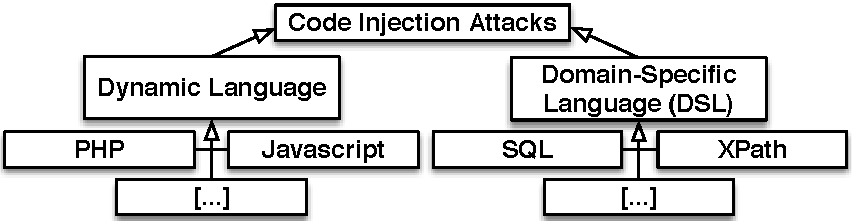
\includegraphics[scale=0.52]{attack-tree-uml.pdf}
\end{center}
\vspace{-6mm}
\caption{\label{fig:taxonomy}A taxonomy of dynamic and domain-specific
language code injection attacks against web applications.}
\vspace{-5.8mm}
\end{figure}

Code injection attacks can be divided in two categories. The first
involves binary code and the second higher-level language code. An
extensive survey on binary code injection attacks was conducted by
Lhee and Chapin~\cite{LC03}. Advances in memory corruption vulnerability
exploitation have been studied extensively~\cite{PB04, SPWS13}
and countermeasures to such attacks
have already been analyzed~\cite{YJP12}.
% \cite[Sec. 13.8]{DKZ12}.
In this work we do not consider binary code injection,
focusing instead on defenses
that protect web applications against attacks based on the
injection of higher-level language code.

Figure~\ref{fig:taxonomy} presents a taxonomy of source
code injection attacks against web applications.
Such attacks may involve high-level language code, written in either a
{\it Domain Specific Language} ({\sc dsl}) or a {\it Dynamic Language}.
To illustrate, we discuss examples from both categories
that will be used throughout the paper.

Injection attacks that involve {\sc dsl}s constitute an important
subset of the code injection problem, as {\sc dsl}s such as
{\sc sql} and {\sc xml} play a significant role in the development of
both web and mobile applications. For example, many applications have
interfaces through which a user enters input to interact with the
application, thereby interacting with the underlying database. This
input can become part of an {\sc sql} query and gets executed on the
target database. Code injection attacks that exploit vulnerabilities
in database interfaces by taking advantage of input validation issues,
such as incorrectly passed parameters or incorrect type handling, are
called {\sc sql} injection attacks~\cite{HVO06,SW06}.
Consider a trivial exploit that takes advantage of incorrectly
filtered quotation characters in an application that shows the
password of a forgetful user by executing the following
query:

\lstset{language=SQL}
\begin{lstlisting}
SELECT password from userdata WHERE id = 'Alice'
\end{lstlisting}

\noindent
Attackers that would input the string {\tt anything' OR 'x'='x}
could view every item in the table.
%obtain a user's password by email.
Savvy programmers can use certain {\sc api} functions, such as {\sc php}'s
{\tt mysql\_real\_escape\_string()}, to detect malformed input, or,
better, use prepared {\sc sql} statements instead of statement
templates. Unfortunately, the increasing number of {\sc sql} injection
attacks suggests that programmers are not always that careful. Using
similar techniques, malicious users can mount other exploits based on
{\sc dsl}s such as {\sc xp}ath~\cite{SW06}, {\sc
  xml}~\cite{MSM13} and {\sc json}~\cite{SMS13}. The effects can be
wide-ranging. A malicious user can view sensitive information, destroy
or modify protected data, or even crash the entire application.

{\sc html} is another {\sc dsl} that can be used for malicious
purposes when an application does not properly handle user-supplied
data. Based on this vulnerability attackers can supply valid {\sc
  html}, typically via a parameter value, and inject their own content
into the application's page. {\sc html} injection is mainly associated
with {\sc xss} attacks~\cite{SLMS14}. However, {\sc html} injection
can also be used as a vehicle for Cross-Site Request Forgery
({\sc csrf}) attacks~\cite{LZRL09}
(even though a common {\sc csrf} attack does not necessarily
involve code injection).
Consider a bulletin board system where {\tt img} tags are allowed.
A malicious user could embed a {\sc csrf} request within an
{\tt img} tag in the following manner:

\lstset{language=HTML}
\begin{lstlisting}
<img src='http://www.vulnerable.com/admin.php?edituserwithID=13&addgroup=admin'/>
\end{lstlisting}

\noindent
When the page with this injected code is accessed by an administrator,
the attacker (with {\sc id} 13) will gain administrative privileges
over the vulnerable.com web page,
while the administrator of the bulletin board system
will have no immediate indication that there has been an attack.

A recent class of code injection attacks involve dynamic languages
such as JavaScript and {\sc php}~\cite{SMS13}.
JavaScript injection attacks make up a large subset of dynamic
language code injection attacks and are considered a critical issue
in web application security mainly because they are associated with
major vulnerabilities such as {\sc xss} attacks~\cite{SG07} and
Cross-Channel Scripting ({\sc xcs}) attacks~\cite{BBB09}.
Such attacks are enabled when a web application accepts
and redisplays data of uncertain origin without
proper validation and filtering. Based on this flaw, an attacker
can manage to inject a script in the JavaScript engine of a browser
and alter its execution flow~\cite{ELX07}.
For a typical {\sc xss} example that involves JavaScript injection
consider a web page that prints the value
of a query parameter ({\tt query}) from the
page's {\sc url} as part of the page's content
without escaping the value. Attackers
can take advantage of this and inject an {\tt iframe} tag
into the page to steal a user's cookie and
send it via an image request to a web site
under their control (malicious.com).
This could be achieved by including the following
link to the malicious web site (or sending it via phishing
email) and inducing the user to click on it:

\lstset{language=HTML}
\begin{lstlisting}
http://example.com/vulnerable.html?query=<iframe src="javascript:document.body.innerHTML=+'<img src=\"http://malicious.com/?c='+encodeURIComponent(document.cookie)+'\">'"></iframe>
\end{lstlisting}

\noindent
Note that in many cases {\sc xss} attacks
involve the injection of both {\sc html} and JavaScript code.

A simple example of a {\sc php} injection attack is an input string
that is fed into an {\tt eval()} function call, e.g.:

\lstset{language=PHP}
\begin{lstlisting}
$variable = $_GET['var']; 
$input = $_GET['value'];
eval('$variable = ' . $input . ';')
\end{lstlisting}

\noindent
The user may pass into the {\tt value} parameter code that will
be executed on the server. Hence, if an attacker provides as
input the following string: {\tt 10 ; system("touch foo");}
then a file will be created on the server---it is easy
to imagine more detrimental scenarios.

A recent attack called {\sc php} Object Injection
({\sc poi})~\cite{DKH14} does not directly involve
the injection of code, but still achieves arbitrary code execution
in the context of a {\sc php} application through the
injection of specially crafted objects.
These objects are injected as part of cookies,
which, when deserialized
by the application, result in arbitrary code execution.
Note that the exploitation model we propose
in the following Section also captures such attacks.

\begin{figure*}[t]
\begin{center}
\leavevmode
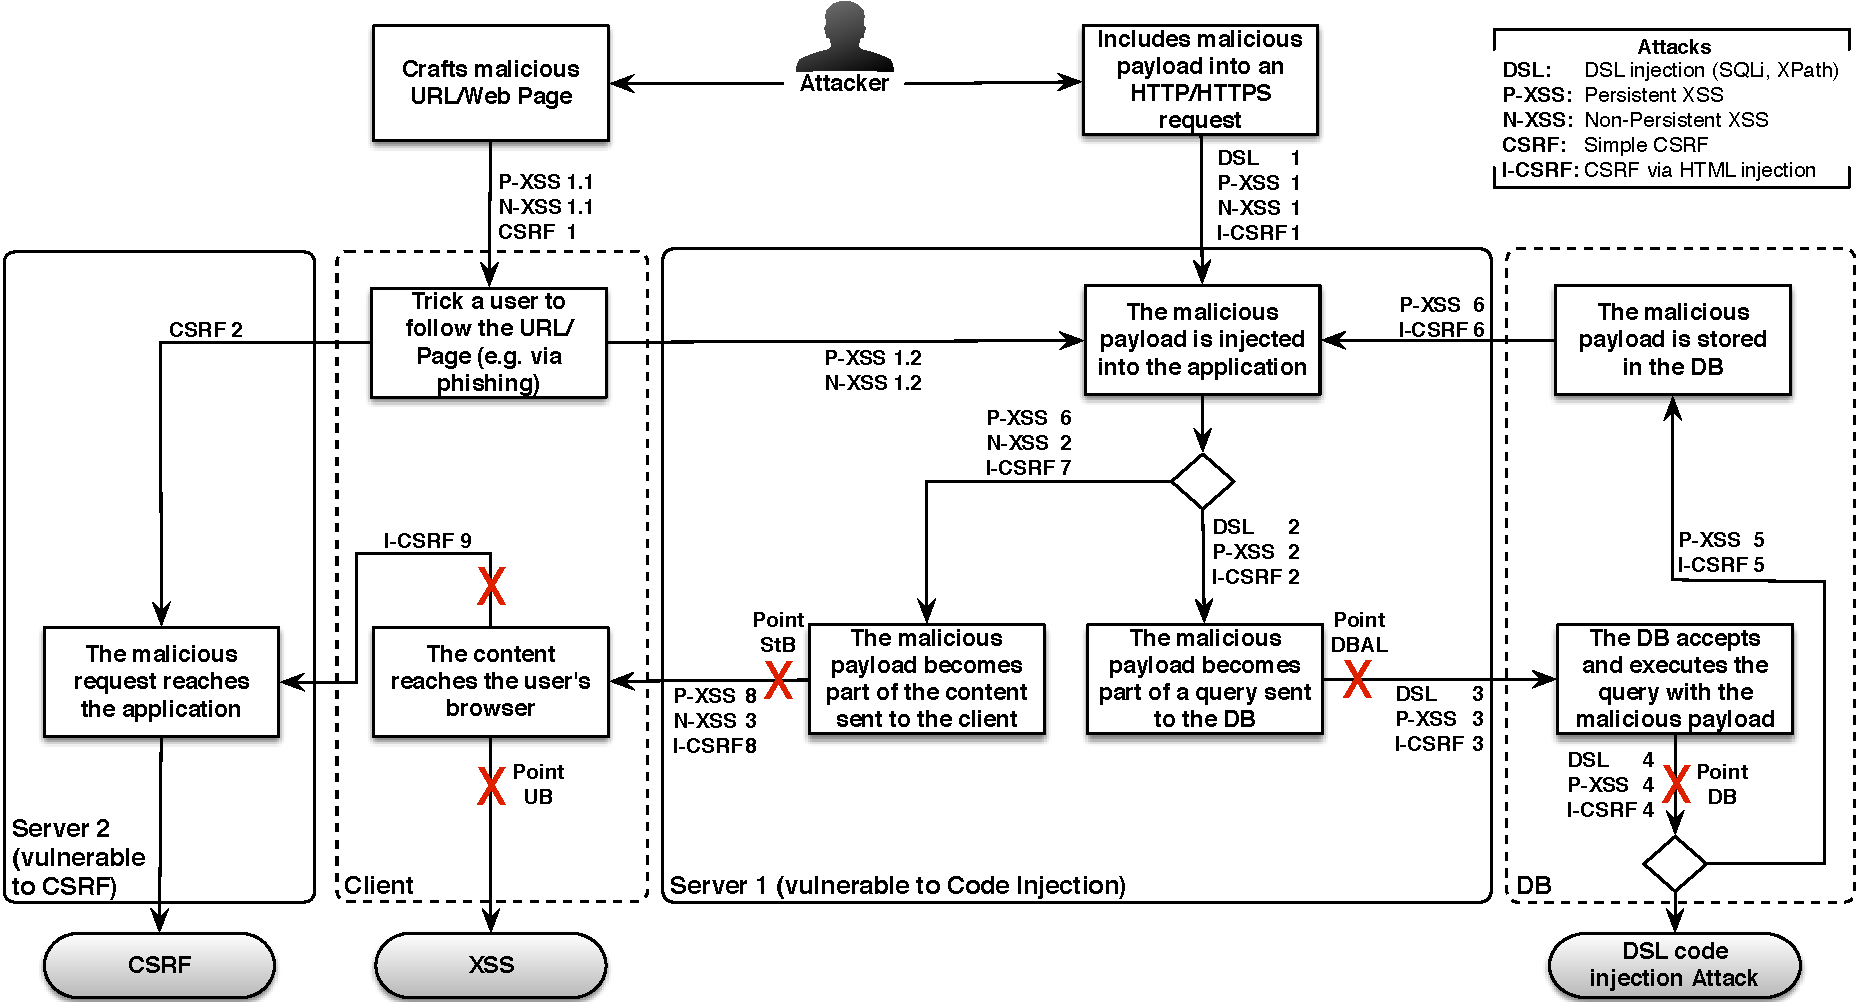
\includegraphics[scale=0.48]{attacks-steps-CSRF.pdf}
\end{center}
\vspace{-5.5mm}
\caption{\label{fig:attacks}Attack model for dynamic and domain specific
language code injection in web applications.
Transitions are labeled with the different attacks that use that path,
while the numbers next to attack labels denote the 
sequence of steps for a particular attack.
Points where different types of defenses
detect or prevent attacks are marked with an `X' symbol:
(1) {\sc ub} (at the browser):~\cite{KJKV09,LV09,TNH07,NSS06,APKLM10,ML10,YCIS07,PSC09,VDDPJ11,OWVS08,DDHPJ10,VFJKKV07,SLMS14,BV08,SSM10},
(2) {\sc s}t{\sc b} (en route from the server to the browser):~\cite{RDWDE07,JKK06a,GC09,JB07,NLC07,WPLKK09,JEP08,PS11},
(3) {\sc dbal} (at the database abstraction layer):~\cite{BWS05,SW06,HCF05,XBS06,PB05,PMP11,MS09,HO05b,SMS13},
(4) {\sc db} (at the database):~\cite{BK04,LLW02,VMV05}.}
\vspace{-6mm}
\end{figure*}

\section{Exploitation Model}
\label{sec:model}

We provide a step-by-step exploitation model to aid in understanding the process
of carrying out code injection attacks against web
applications. Figure~\ref{fig:attacks} illustrates the required steps for
different classes of attacks,
such as {\sc sql} injection, {\sc xss}, and {\sc csrf}. Links between steps are
labeled with the different attacks that use that path, while the
numbers next to attack labels denote the sequence of steps for a
particular attack. Most steps are common in all attacks, as different attack
types follow similar exploitation paths, as mentioned in
the previous section. Large `X' marks on transitions correspond to the
points where the defenses we consider in this work detect or prevent attacks.

An attacker can initiate an injection attack through two main routes.
One way is to use the browser of a victim as an attack
vehicle, through which the code will be injected in the application.
For example, the attacker could embed a malicious script into a {\sc
  url} and then trick a user to click on it through social
engineering, e.g., by sending a phishing email (transition {\sc p-xss} 1.1, {\sc
  n-xss} 1.1, {\sc csrf} 1). Alternatively, the attacker may be able
to inject directly the malicious code on the server through an {\sc http} request
({\sc dsl} 1, {\sc p-xss} 1, {\sc n-xss} 1, {\sc i-csrf} 1). This would happen
in a web application that accepts and processes user input
without appropriate validation. An attacker could upload data
containing a specially crafted script
to steal the cookies of the visiting users ({\sc p-xss} 1, {\sc n-xss} 1),
an {\tt img} tag including a malicious {\sc http} request ({\sc csrf 1}, {\sc
i-csrf 1}),
or embed malicious
{\sc sql} code to retrieve private data from a database ({\sc dsl} 1).
Note that, {\sc xss} and {\sc csrf} attacks can start from both routes.
Once the injected code reaches the vulnerable application, it becomes
a part of a value represented by a program variable. The target of the
attack determines the route from that point and on. In an {\sc sql} injection
attack, the injected code becomes part of a query that
eventually reaches the database where it is executed.

Cross-site scripting attacks fall into two categories, {\it non-persistent}
(also known as \emph{reflected}) {\sc xss}
and {\it persistent} (also known as \emph{stored}) {\sc xss}.
Non-persistent {\sc xss} attacks take place when the
data provided by a user is processed on-the-fly
by server-side application logic and ends up without proper sanitization
into a dynamically generated response ({\sc p-xss} 7, {\sc n-xss} 2)
that is eventually rendered by the user's browser.
Thus, in a non-persistent {\sc xss} attack, the injected code
is not saved on the server, but immediately becomes part of the
content that is sent back to a user.
In persistent {\sc xss} attacks, on the other hand,
malicious code is permanently stored on the server ({\sc p-xss} 5).
The injected code residing at server-side then re-enters the
application's execution flow and becomes part of the content that is
eventually sent to the user as part of a future response.

{\sc csrf} attacks typically involve just a
{\sc url} or page that contains a malicious request towards
a site vulnerable to {\sc csrf}.
An attacker can entice a victim to click on the {\sc url} or visit the page
through social engineering ({\sc csrf} 1), which will the result in a malicious
request towards the vulnerable site ({\sc csrf} 2).
Note that this scenario does not involve the injection of any code through the
exploitation of some server-side vulnerability (as is the case with Server 1).
On the other hand, {\sc csrf} is also possible through injection
({\sc i-csrf}---recall our example in the previous section).
In this attack, an attacker
manages to inject {\sc html} code that contains
a malicious {\sc csrf} request in the way we described in
Section~\ref{sec:attacks}.
This code will be stored
in the database ({\sc i-csrf} 5)
and then it will re-enter the application when
a user visits a page ({\sc i-csrf} 6). When the
content reaches the browser, a malicious request will be generated
towards the site that is vulnerable to {\sc csrf}.

\section{Analysis Dimensions}
\label{sec:dimensions}

Research on web application attack defense mechanisms has a dual
character. First, a defense mechanism may be important, and therefore
publishable, because it shows that an attack can be detected or prevented in a
reliable manner. Second, a defense mechanism may be important not
just as a research contribution, but as a practical tool, if it can be
used by administrators and users to shield their applications
against the supported attacks.

The detection and prevention of attacks
in a reliable manner can be analyzed using
criteria common with other research fields:
\begin{itemize}
\item Statistical measurements that show how
reliable the detection really is.
\item Research practices that promote replication and validation
of the findings.
\end{itemize}

\noindent
Whether a reliable defense mechanism has value in a practical
setting rests on a different set of criteria:
\begin{itemize}
\item What are the overheads imposed by the mechanism?
\item How easy is it to deploy and use the mechanism?
\item How robust is it against ways to circumvent it?
\item At which point throughout the system does it block an attack?
\end{itemize}

The first two criteria correspond to \emph{Accuracy} and
\emph{Availability}. The other four criteria correspond to \emph{Runtime
  Performance}, \emph{Ease of Use}, \emph{Security}, and
\emph{Point of Detection}.

\subsection{Accuracy}
\label{ssec:diagnostic-performance}

Web application defenses 
crucially have to capture the presence of an attack. This, however, does not
make a defense mechanism immediately useful. A
detection mechanism must also be reliable.
Detection accuracy is gauged with the following
metrics~\cite{GFDLS06,A00}:
\begin{itemize}
\item {\bf Sensitivity}: the probability that an attack will be
  caught.
\item {\bf Specificity}: the probability that a normal interaction
  will not be flagged.
\item {\bf Positive Predictive Value} ({\sc ppv}): the probability that a
  reported attack is a real attack. It is the conditional probability
  that an event is an attack if the detection mechanism flags it as
  such. 
\item {\bf Negative Predictive Value} ({\sc npv}): the probability that if
  nothing is reported, no attack has taken place. It is the conditional
  probability that an event is not an attack given that the detection
  mechanism flags it as normal.
\end{itemize}

\noindent
We will focus on sensitivity and specificity; we will come back to
\textsc{ppv} and \textsc{npv} in Section~\ref{sec:lessons-learned}.
Sensitivity and specifity are defined as follows~\cite{linn2004}:
\begin{itemize}
\item True Positive (\textsc{tp}): an attack that raises an alarm.
\item True Negative (\textsc{tn}): an event that is not an attack and that does
  not raise an alarm.
\item False Positive (\textsc{fp}): an event that although it is not an attack,
  raises an alarm.
\item False Negative (\textsc{fn}): an event that although is an attack, does
  not raise an alarm.
\end{itemize}

\noindent
With these we can calculate:

\vspace{0.5mm}
\noindent\begin{minipage}{0.5\linewidth}
\begin{equation}
  \textsc{se} = \textrm{Sensitivity} = \frac{\textsc{tp}}{\textsc{tp}
    + \textsc{fn}}
\label{eq:sensitivity}
\end{equation}
\end{minipage}%
\begin{minipage}{0.5\linewidth}
\begin{equation}
  \textsc{sp} = \textrm{Specificity} = \frac{\textsc{tn}}{\textsc{fp}
    + \textsc{tn}}
\label{eq:specificity}
\end{equation}
\end{minipage}\par\vspace{\belowdisplayskip}

\noindent
Sensitivity and specificity can be calculated based on test
data alone. To calculate sensitivity, we run the test on a
controlled environment where we allow only attack events to reach the
system. The ratio of reported attacks over all attacks will give us
the sensitivity. Similarly, to calculate the specificity we can run
the test on a controlled environment where we allow only innocuous
events to reach the system. The ratio of non-reported events over all
events will give us the specificity.
Note that the use of sensitivity and specificity in this context
has been advocated before~\cite{PP12}.

\subsection{Availability}

To ensure reproducibility of research results, the source code
implementing a detection mechanism should be available to researchers.
Ideally the code should be available under an open source license, so
that it is easy to modify and improve an approach; even when this is
not possible, for whatever reason, it is important to make sure that
all computer code and test data is available, noting any restrictions
on accessibility. Availability of computer code has been recognized as
an important issue outside the computer science field: the journal
\emph{Nature}, in a recent editorial, adopted a publication policy stressing
access to code and data~\cite{nature2014}. At a time and date that the
merits of open access to code are discussed in non computer science
journals~\cite{easterbrook2014}, we should expect computer scientists
to lead the way.
 
\subsection{Performance Overhead}

Detection mechanisms may impose a cost due to their use, as they
typically introduce some amount of extra computation on existing applications.
The overhead depends on the specifics of each mechanism. For
example, it may be due to some form of run-time checking, or some form of
obfuscation. Also, depending on the approach, the cost may be incurred
on different places: it may affect a server
(e.g., its memory or {\sc cpu} usage, processing throughput, or response latency),
it may affect the client, or both. The
usefulness of a mechanism depends therefore on the
computational cost it requires and on where it imposes it, as
different overheads may be acceptable at the server-side than the client-side.
What kind of numbers is reported matters as well. Reporting absolute
measurements gives little information on the actual overhead, unless
separate measurements are given for the system under study with and
without the proposed mechanism. Percentage measurements are normally
better. 

Performance evaluation rests on strong foundations~\cite{jain1991} and
is a vibrant field as new technologies emerge~\cite{gregg2014}.
Although it may not be necessary to conduct a comprehensive
performance evaluation analysis for a defense mechanism, the more
evaluation results are provided for a mechanism, the more valuable
it becomes as a practical approach.

\subsection{Ease of Use}
\label{sec:deployment}

The value of a detection mechanism as a practical tool depends on how
easy it is to deploy it in a production setting. This aspect is
orthogonal to the
value of a detection mechanism as a research finding. Devising a
technique to detect a hitherto undetectable class of attacks may be an
excellent research contribution that merits publication; it may also
be heavily cited and open the road to other, practical
implementations in the future. 

Ease of use depends on the deployment process required for the
mechanism. The detection mechanism may be deployed at either or both
the server and the client-side. Deployments on just the server or the client are
easier to handle than deployments on both of them. The mechanism may
be an add-on or plugin for existing software, client or server, or it
may be tightly integrated with existing software, requiring rebuilding
from source code.

No matter where it is installed, the means of installation influences
ease of use. A detection mechanism that is available as a ready-to-install
package will trump others that only exist in the form
of source code. 

\subsection{Security}

Defenders and attackers are often caught in a cat-and-mouse game,
where countermeasures are bypassed by canny attacks, which are caught
by more sophisticated countermeasures, yet again bypassed by cannier
attacks, and so on. We use security to refer to the ability of a
detection mechanism to resist circumvention. 

A mechanism that has not been bypassed is not eternally secure, as it
is possible that a bypass method will be discovered in the future. We
examine the various approaches based on the knowledge we have so far,
that is, whether there are any known ways to bypass the detection
mechanism today.

\subsection{Point of Detection}
\label{sec:point}

Detection mechanisms vary on the location where they detect an attack.
There are four different points where an attack can be caught, as seen
in Figure~\ref{fig:attacks}:
\vspace{-0.5mm}
\begin{enumerate}
\item At the user's browser (Point {\sc ub}).
\item En route from the server to the user's browser---in most cases
within a proxy (Point {\sc s}t{\sc b}).
\item At the database abstraction layer, before it reaches the server's database
  (Point {\sc dbal}).
\item After the malicious code reaches the server's database
  (Point {\sc db}).
\end{enumerate}
\vspace{-0.5mm}

\begin{figure}[t]
\begin{center}
\leavevmode
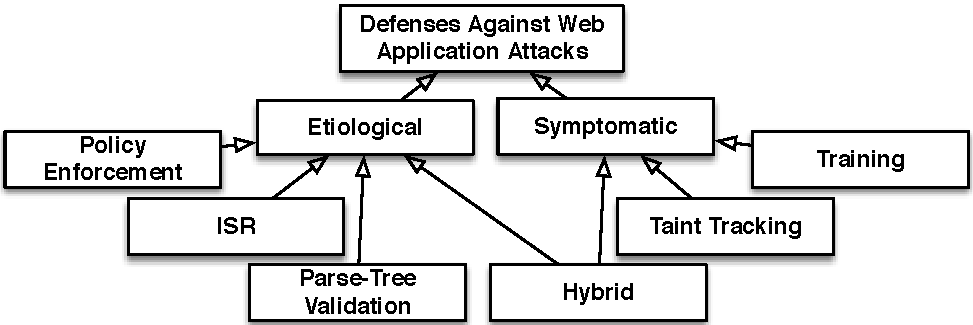
\includegraphics[scale=0.53]{defenses.pdf}
\end{center}
\vspace{-5.8mm}
\caption{\label{fig:defenses}The basic categories of countermeasures
against web application attacks based on code
injection. For each approach we provide the references
that present corresponding mechanisms:
{\it Policy Enforcement}:~\cite{NSS06,JKK06a,KJKV09,TNH07,RDWDE07,YCIS07,OWVS08,PSC09,ML10,DDHPJ10,PS11,VDDPJ11,BV08,SSM10},
{\sc isr}:~\cite{BK04,JB07,GC09,APKLM10},
{\it Parse-Tree Validation}:~\cite{BWS05,SW06},
{\it Taint Tracking}:~\cite{HCF05,PB05,XBS06,NLC07,VFJKKV07,PMP11,SLMS14},
{\it Training}:~\cite{LLW02,HO05b,VMV05,JEP08,WPLKK09,MS09,MKLS11},
{\it Hybrid}:~\cite{BV08,LV09,SMS13}.}
\vspace{-5.5mm}
\end{figure}

\begin{table*}[t]
  \renewcommand{\baselinestretch}{1.12}
    \caption{Comparison summary of mechanisms developed to counter application attacks based on code injection.}
    \label{tab:comp}
    \vspace{-4.5mm}
\centering
    \begin{threeparttable}
    \begin{small}
\scalebox{0.78}{
    \begin{tabular}{l|c|c|cc|c}
    \thickhline
    \bf{Approach}
  & \bf{Mechanism}
  & \bf{\# of Citations}
  & \multicolumn{2}{c|}{Requirements\tnote{1}}
  & \bf{Attack}\tnote{4} \\
  &&& \bf{TP,TN,FP,FN}\tnote{2}
  & \bf{Performance Overhead}\tnote{3} & \\
    \thickhline
  \multirow{2}{*}{Parse-Tree Validation}
  &   {\sc sqlg}uard~\cite{BWS05} & 305 & ({\sc na},{\sc na},{\sc na},{\sc na})\_{\bf ?} & 3\% ({\sc s}) & {\sc sql}i \\
  &   {\sc sqlc}heck~\cite{SW06} & 473 & (36848,7648,0,0)\_r & 3ms per query ({\sc s}) & {\sc sql}i \\
  \hline
  \multirow{13}{*}{Policy Enforcement}
  &   {\sc dsi}~\cite{NSS06} & 168 & (5268,{\sc nq},{\sc nq},85)\_r & 1.85\% ({\sc c}) & {\sc xss} \\ 
  &   NoForge~\cite{JKK06a} & 151 & (7,{\sc nq},{\sc nq},0)\_r & {\sc na} ({\sc s}) & {\sc csrf} \\
  &   Noxes~\cite{KJKV09} & 58 & (3,{\sc na},{\sc na},0)\_r & {\sc na} ({\sc c}) & {\sc xss} \\
  % &   {\it {\sc met}}~\cite{ELX07} & 58 & ({\sc na},{\sc na},{\sc na},{\sc na})\_{\bf ?} & {\sc na} & {\sc xss} \\ 
  &   {\sc beep}~\cite{TNH07} & 335 & (61,{\sc na},{\sc na},0)\_r & 14.4\% ({\sc c}) & {\sc xss} \\
  &   BrowserShield~\cite{RDWDE07} & 263 & (19,{\sc nq},0,0,)\_r & 8\% ({\sc s}) & {\sc xss} \\ 
  &   CoreScript~\cite{YCIS07} & 199 & ({\sc nq},{\sc nq},{\sc nq},{\sc na})\_s & {\sc nq} ({\sc c}) & {\sc xss} \\
  &   {\it {\sc soma}}~\cite{OWVS08} & 56 & (5,{\sc na},{\sc na},0)\_s & 5.58\% ({\sc c}) & {\sc xss}, {\sc csrf} \\
  % &   {\it Barth et al.}~\cite{BJM08} & 271 & & {\bf ?} & {\sc csrf} \\
  &   Phung et al.~\cite{PSC09} & 101 & (37,{\sc na},{\sc na},4)\_r & 5.37\% ({\sc c}) & {\sc xss} \\
  &   ConScript~\cite{ML10} & 152 & ({\sc na},{\sc na},{\sc na},{\sc na})\_{\bf ?} & 7\% ({\sc c}) & {\sc xss} \\
  &   CsFire~\cite{DDHPJ10} & 46 & (419582,1141807,0,3)\_r\tnote{5} & {\sc na} ({\sc c}) & {\sc csrf} \\
  &   {\sc csp}~\cite{SSM10} & 117 & ({\sc na},{\sc na},{\sc na},{\sc na})\_{\bf ?} & {\sc nq} ({\sc c}) & {\sc xss}, {\sc csrf} \\
  &   j{\sc csrf}~\cite{PS11} & 4 & (2,{\sc na},{\sc na},0)\_r & 2ms ({\sc s}) & {\sc csrf} \\
  &   WebJail~\cite{VDDPJ11} & 45 & (2,{\sc na},{\sc na},1)\_{\bf ?} & $\sim$6.89ms ({\sc c}) & {\sc xss} \\
  % &   {\it TreeHouse}~\cite{IW12} & 18 & ({\sc na},{\sc na},{\sc na},{\sc na})\_{\bf ?} & 757–-1218ms & {\sc xss} \\
  % &   {\it {\sc js}and}~\cite{AVBPDP12} & 22 & ({\sc na},{\sc na},{\sc na},{\sc na})\_{\bf ?} & up to 31.2\% & {\sc xss}\\
  % \hline
  % \hline 
  % \multirow{3}{*}{Securing Mashups}
  % &   {\it {\sc om}ash}~\cite{CHC08} & 58 & ({\sc na},{\sc na},{\sc na},{\sc na})\_{\bf ?} & {\sc nq} & {\sc csrf} \\
  % &   {\it Mashup{\sc os}}~\cite{WFHJ07} & 149 & ({\sc na},{\sc na},{\sc na},{\sc na})\_{\bf ?} & 1--59\% & {\sc xss} \\
  \hline
  \multirow{4}{*}{{\sc isr}}
  &   {\sc sql}rand~\cite{BK04} & 365 & (3,{\sc na},{\sc na},0)\_a & $\le$6.5{\it ms} ({\sc s}) & {\sc sql}i \\
  &   {\sc sm}ask~\cite{JB07} & 28 & (5,{\sc nq},{\sc nq},{\sc nq})\_r  & {\sc na} ({\sc s}) & {\sc sql}i, {\sc xss} \\
  &   Noncespaces~\cite{GC09} & 132 & (6,{\sc na},{\sc na},0)\_r &  2\% ({\sc s}) & {\sc xss} \\ 
  &   x{\sc js}~\cite{APKLM10} & 20 & (1380,{\sc na},{\sc na},1)\_r & 1.6--40{\it ms} ({\sc c}) & {\sc xss} \\
  \thickhline
  \thickhline
  \multirow{7}{*}{Taint Tracking}
  &   Haldar et al.~\cite{HCF05} & 208 & (2,{\sc na},{\sc na},0)\_s & {\sc nq} ({\sc s}) & {\sc sql}i, {\sc xss} \\ 
  &   {\sc csse}~\cite{PB05} & 347 & (7,{\sc nq},{\sc nq},{\sc nq})\_r & 2--10\% ({\sc s}) & {\sc sql}i, {\sc xp}athi, {\sc xss} \\
  % &   {\it SecuriFly}~\cite{MLL05} & 31 & \xmark,\tick & 9--125\% & {\sc sql} injection, {\sc xss} \\ 
  &   Xu et al.~\cite{XBS06} & 346 & (9,{\sc nq},0,{\sc nq})\_r & average 76\% ({\sc s}) & {\sc sql}i, {\sc xss} \\ 
  &   {\sc wasc}~\cite{NLC07} & 32 & ({\sc nq},{\sc nq},{\sc nq},{\sc nq})\_r & up to 30\% ({\sc s}) & {\sc sql}i, {\sc xss} \\
  &   Vogt et al.~\cite{VFJKKV07} & 400 & ({\sc nq},{\sc nq},{\sc nq},{\sc na})\_r & {\sc nq} ({\sc c}) & {\sc xss} \\
  &   {\sc php} Aspis~\cite{PMP11} & 20 & (12,{\sc nq},{\sc nq},2)\_r & 2.2$\times$ ({\sc s}) & {\sc sql}i and {\sc php}i, {\sc xss} \\
  &   Stock et al.~\cite{SLMS14} & 15 & (1169,{\sc na},{\sc na},0)\_r & 7--17\% ({\sc c}) & {\sc dom}-based {\sc xss} \\
  \hline 
  \multirow{6}{*}{Training}
  &   {\sc didafit}~\cite{LLW02} & 190 & ({\sc na},{\sc na},{\sc na},{\sc na})\_{\bf ?} & {\sc na} ({\sc s}) & {\sc sql}i \\
  &   {\sc amnesia}~\cite{HO05b} & 474 & (1470,{\sc nq},0,0)\_a & {\sc nq} ({\sc s}) & {\sc sql}i \\ 
  &   libAnomaly~\cite{VMV05} & 259 & (9,15987,60,0)\_r & 0.20--1{\it ms} per query ({\sc s}) & {\sc sql}i \\
  &   {\sc xssds}~\cite{JEP08} & 85 & ({\sc nq},{\sc nq},{\sc nq},0)\_r & {\sc nq} ({\sc s}) & {\sc xss} \\
  &   {\sc swap}~\cite{WPLKK09} & 68 & ({\sc nq},{\sc nq},{\sc nq},{\sc nq})\_r & up to 261 {\it ms} ({\sc s}) & {\sc xss} \\ 
  &   {\sc sd}river~\cite{MS09,MKLS11} & 28 & (241,{\sc nq},0,0)\_a & 39\% ({\sc s}) & {\sc sql}i and {\sc xp}athi \\
  % &   {\it Laranjeiro et al.}~\cite{LVM09,ALVM09,LVM10} & 9,40,1 & \xmark,\xmark  & \xmark & {\sc sql} and {\sc xp}ath injection \\
  \thickhline
  \thickhline
  \multirow{3}{*}{Hybrid}
  &   {\sc xss-guard}~\cite{BV08} & 132 & (8,{\sc nq},{\sc nq},{\sc nq})\_r & 5--24\% ({\sc c}) & {\sc xss} \\
  &   Blueprint~\cite{LV09} & 152 & (94,{\sc na},{\sc na},0)\_r & 13.6\% ({\sc c}) & {\sc xss} \\
  &   Diglossia~\cite{SMS13} & 13 & (25,{\sc nq},{\sc nq},{\sc nq})\_r & 13\% ({\sc s}) & {\sc sql}i and {\sc json}i \\
  \thickhline
    \end{tabular}}
    \begin{tablenotes}
  \begin{footnotesize}
        \item[1] {\sc na} (Not Available) indicates that a requirement is not mentioned in the paper.
  {\sc nq} (Not Quantified) indicates that a requirement is mentioned in the\newline publication
  but is not quantified.
      \item[2] Tuples contain numbers given for True Positives
        ({\sc tp}), True Negatives ({\sc tn}), False Positives ({\sc
          fp}) and False Negatives ({\sc fn}). For every tuple\newline there is a corresponding suffix that indicates whether the testbed was
  based on: real-world applications known to be vulnerable ({\it r}),
  synthetic\newline benchmarks ({\it s}), or both ({\it a}).
  A question mark ({\bf ?}) denotes that no test results are reported.
    \item[3] Whether the overhead is incurred on the server ({\sc s}) or the client ({\sc c}). 
    \item[4] {\it i} stands for injection.
    \item[5] The numbers in this particular case involve requests.
  \end{footnotesize}
    \end{tablenotes}
    \end{small}
    \end{threeparttable}
    \vspace{-6.7mm}
\end{table*}

\section{Defenses}
\label{sec:defs}

We categorize and analyze a large set of defenses developed to prevent
the attacks described in Sections~\ref{sec:attacks} and~\ref{sec:model}.
We perform our analysis across
the dimensions discussed in the previous section,
except from availability, which we treat
separately in Section~\ref{sec:discussion}.
Due to the immense number of published works in the area, we only consider
defenses that have been proposed in publications cited more than
20 times according to Google Scholar.
We also include some recent works that have been
presented in top security conferences, even though they have been
cited less than twenty times, so that recent research is not penalized.

Figure~\ref{fig:defenses} presents a taxonomy of 
web application defenses against injection attacks.
We can identify three broad categories:
{\it etiological}, {\it symptomatic}, and {\it hybrid}.
The etiological category involves mechanisms designed to
block attacks based on their causes and origins~\cite{L81}. 
The symptomatic category incorporates a variety of schemes that
inspect the behavior of applications and detect attacks based on
their undesirable symptoms~\cite{D76,A00}.
Hybrid mechanisms borrow characteristics from both
categories. Table~\ref{tab:comp} lists the specific mechanisms we consider
in this work, grouped according to the subcategories shown in
Figure~\ref{fig:defenses}, and for each mechanism
provides the following information:

\vspace{-0.5mm}
\begin{enumerate}
\item Number of citations of the corresponding publication(s).
\item Accuracy and computational overhead measurements.
\item Types of attacks handled.
\end{enumerate}
\vspace{-0.5mm}
\noindent
Recall that the point of operation for each mechanism is provided
in the caption of Figure~\ref{fig:attacks}.

\subsection{Etiological}
\label{sec:prot}

There are three main categories of etiological approaches used to protect web
applications against injection attacks:
\emph{Parse-Tree Validation},
\emph{Policy Enforcement}, and
\emph{Instruction Set Randomization} ({\sc isr}).

\subsubsection{Parse-Tree Validation}
\label{sec:tree}

The key idea behind parse-tree validation is to compare the tree
representation of the abstract syntactic structure of the code
that is about to be executed with the one that was originally
intended. If the trees diverge, the application is probably under
attack.

For {\sc dsl} code injection attacks, mechanisms check 
the query before the inclusion of user input with the one
resulting after the inclusion of user input.
Two mechanisms that implement this approach for protection
against {\sc sql} injection attacks,
{\sc sqlg}uard~\cite{BWS05} and
{\sc sql}check~\cite{SW06}, are quite similar
and detect the attack before a query reaches the
database (Point {\sc dbal}).
Contrary to {\sc sqlg}uard,
% mikepo: if others exist, cite them
%and other mechanisms,
{\sc sql}check has been
extensively tested in terms of accuracy,
as can be seen in Table~\ref{tab:comp}.
A disadvantage of these mechanisms is that the
application must be modified in every code fragment
that sends an {\sc sql} query to the database for execution.

Parse-tree validation is an effective approach
for the detection of {\sc dsl} code injection attacks,
especially as implemented in {\sc sql}check.
This is not however the case
for mechanisms that borrow elements from
this approach and examine the syntax trees
of scripts to detect JavaScript-driven {\sc xss} attacks,
as we will see in Section~\ref{sec:hybrid}.

\subsubsection{Policy Enforcement}
\label{sec:policy}

This approach is used to prevent {\sc xss} and {\sc csrf} attacks. When
using a framework that implements policy enforcement, developers must
define specific security policies on the server-side. Policies can be
expressed through JavaScript extensions, pattern matching, or
syntax-specific settings. The policies are then enforced either in the user's
browser at runtime, or on a server-side proxy that intercepts server
responses.

Noxes~\cite{KJKV09} is the only
framework that partially allows
users to specify policies for the prevention of {\sc xss} attacks.
The key idea behind Noxes is to parse
the {\sc html} response that reaches the browser and
find static {\sc url} references. Then, based on
a set of policies, Noxes allows or blocks
any generated requests (Point {\sc ub}). Such policies
can also be provided by the server (i.e., ``never
follow a link that leads to the malicious.com
web site''). The main issue with Noxes is that
{\sc url}s can be dynamically assembled by scripts,
which may lead to false alarms.

Some frameworks define policies based on information and
features provided by the Document Object Model ({\sc dom}) of a web
page. Specifically, developers must place all legitimate scripts
inside {\sc html} elements like {\tt div}. The web browser (Point {\sc
  ub}) parses the {\sc dom} tree and executes scripts only when they
are contained in such elements. All other scripts are treated
according to the policies defined on the server. Frameworks that
support this functionality include {\sc beep}~\cite{TNH07} and {\sc
  dsi}~\cite{NSS06}. The main problem with these mechanisms is that
they do not examine the script's location inside the web document.
Attackers can take advantage of this fact to perform mimicry attacks~\cite{WS02}.
Specifically, they can execute legitimate scripts, but not as intended
by the original design of the developers. This is extensively
described by Athanasopoulos et al.~\cite{APKLM10}, who also describe
another recent variation of JavaScript injection attacks, known as
return-to-JavaScript attacks, which can be used to bypass the above
mechanisms.
\vspace{-0.5mm}

A policy enforcement technique developed by Mozilla,
called {\sc csp} (Content Security
Policy)\footnote{\scriptsize\url{https://developer.mozilla.org/en-US/docs/Web/Security/CSP}}~\cite{SSM10}
is currently supported by many browsers to prevent
{\sc xss} and {\sc csrf} attacks. To eliminate such
attacks, web site administrators
can specify which domains the browser should treat
as valid sources of script and which not. Then, the browser
(Point {\sc ub}) will only execute scripts that exist in
source files from white-listed domains.
Note that,
if an application involves
embedded scripts, developers must utilize
the {\sc csp}'s {\em nonce} concept.
This is an unpredictable,
random value indicated in
the {\tt script-src} directive which in turn,
is applied as a nonce attribute to
{\tt <script>} elements.
As a result, only those elements that have the
correct nonce will execute.
Even if an attacker
is able to inject markup into the page,
the attack will be prevented by the attacker's
inability to guess the nonce value.
However, attackers may still bypass this feature
and invoke a script from a non-whitelisted source.
To do so, their injected code must
be crafted in a way that the nonce is handled
by the browser as an attribute of the payload~\cite{jigsaw}.
\vspace{-0.5mm}

Another policy enforcement approach introduces
policies directly either in {\sc html} or JavaScript code
to confine their behavior. BrowserShield~\cite{RDWDE07}
acts as a proxy on the server-side (Point {\sc s}t{\sc b}) to
parse the {\sc html} of server responses and identify
scripts. Then, it rewrites them into safe equivalents
and protects the web user from exploits
that are based on reported browser vulnerabilities.
ConScript~\cite{ML10}, CoreScript~\cite{YCIS07},
and the framework by Phung et al.~\cite{PSC09}
extend JavaScript with new primitive functions that
provide safe methods to protect potentially vulnerable
JavaScript functions. In both cases, policy enforcement takes
place at client-side, in the JavaScript engine of the browser (Point {\sc ub}).
In this way, {\sc xxs} attacks that take advantage
of functions such as {\tt write} and {\tt eval}, which are
used to assemble innocuous-looking parts into harmful
strings,\footnote{\scriptsize The infamous Sammy worm that
infected MySpace in 2005~\cite{ELX07}
utilized the {\tt eval} function to assemble a
malicious script.} would fail.

An issue regarding the above frameworks
involves features like script inclusion
and {\tt iframe} tags. Even though they allow developers
to decide if they will disable them or not,
this is impractical because such features are quite popular and widely used.
If developers choose to use them, these frameworks cannot
define policies that restrict the behavior of third-party
scripts introduced by such features. Thus, they would
be vulnerable to attacks that use {\tt iframes}
in the way described in Section~\ref{sec:attacks}.
WebJail~\cite{VDDPJ11}, and {\sc soma}~\cite{OWVS08}
are two frameworks that can actually detect such attacks (Point {\sc
  ub}). To achieve this, {\sc soma} requires site administrators to
specify legitimate, external domains for sending or receiving
information in order to approve interactions between them and the
protected web site. As a result, {\sc soma} can also detect {\sc csrf}
attacks. WebJail contains the functionality of third-party scripts by
introducing a web component integrator that restricts the access that
these scripts may have to either the data or the functionality of
other components.

Policy enforcement mechanisms that detect {\sc csrf}
attacks are usually implemented in the form of a
server-side proxy (Point {\sc s}t{\sc b})
interposed at the client-server communication path.
NoForge~\cite{JKK06a}
parses the {\sc html} server responses
and adds a token to every {\sc url} referring to that particular
server. Then, it associates the token with the cookie
representing the session {\sc id} for the application.
When a request is received, the mechanism checks
if the request contains the token related
to the session {\sc id}. A disadvantage of NoForge
is that  dynamically created {\sc html} within
the browser will not include the token.
Thus, sites that create part of their {\sc html} code at client-side
will remain vulnerable. In addition, it does not
support cross-origin requests.
The above problems are addressed by j{\sc csrf}~\cite{PS11},
which shares similar functionality.
Finally, CsFire~\cite{DDHPJ10}
examines cross-domain interactions to design a
cross-domain policy at the client-side (Point {\sc ub}).
The policy is based on the concept of a relaxed
same-origin policy that allows communication between
sub-domains of the same registered domain.

Most of the above frameworks involve
several deployment hurdles, as they
require significant source code modifications by the
developers on the server-side to introduce and enforce
the applied policies.

\subsubsection{Instruction Set Randomization (ISR)}

{\sc isr} is a method that has been applied to counter different kinds
of application attacks~\cite{K09b}, and was originally applied for the
prevention of binary code injection attacks~\cite{KKP03}.
The main idea behind {\sc isr} is
to change the representation of code
based on a randomly chosen transformation,
and randomizing the execution environment accordingly.
In this way, any malicious code injected as part of untrusted input data,
by attackers who do not know the randomization algorithm,
will not be executed.

{\sc sql}rand~\cite{BK04} applies the concept of {\sc isr} for the prevention
of {\sc sql} injection attacks. It allows programmers to create {\sc sql}
statements using randomized instructions instead of standard keywords.
The modified queries are reconstructed at runtime using the same key
used for randomization, which is inaccessible to a malicious user.
{\sc sql}rand is one of the few mechanisms that prevent {\sc sql}
injection attacks at the database level (Point {\sc db}).

The same concept can be applied for protection against
{\sc xss} attacks that inject JavaScript or {\sc html} code.
Initially, the trusted code of a web page can be transformed
to a random representation using a simple function such as {\sc xor}.
Before being sent to the client (Point {\sc s}t{\sc b}),
or being processed by the browser (Point {\sc ub}),
the legitimate code is transformed back to its original form,
while any additional injected code will be transformed into junk code.
Variations of this approach include
Noncespaces~\cite{GC09} and x{\sc js}~\cite{APKLM10}, which
randomize the instruction set of {\sc html} and JavaScript,
respectively. Contrary to x{\sc js}, in Noncespaces administrators
must set specific policies in a manner similar to a firewall
configuration language. {\sc sm}ask~\cite{JB07} is another
framework that was inspired by {\sc isr}. To detect {\sc xss}
attacks, it searches for {\sc html} and
JavaScript keywords within the application's legitimate code. This is
done before the processing of any {\sc http} request. When a keyword is found,
it adds a token to it, resulting in a ``code mask.'' Then, before
sending the resulting {\sc html} data to the user, the framework
searches the data for illegal code using the same keywords (Point
{\sc s}t{\sc b}). Since all legitimate code has been ``masked,'' the injected
code can be identified. The need for 
pre-processing and post-processing the code,
however, may add a significant overhead to the application.
Unfortunately, the authors of {\sc sm}ask did not provide measurements
regarding the runtime overhead of the tool (see
Table~\ref{tab:comp}).

{\sc isr} is a deterministic approach that can be applied to prevent
different attacks in an effective manner. However, Sovarel et
al.~\cite{SEP05} have investigated thoroughly the effectiveness of
{\sc isr} and showed that a malicious user may be able to circumvent
it by determining the randomization key. Their results indicate
that applying {\sc isr} in a way that provides a certain degree of
security against a motivated attacker is more difficult than
previously thought. Furthermore, developers who wish to use such
mechanisms must follow good coding practices and make sure that
randomized code statements are never leaked
(e.g., as part of an exception error),
as this may be used to reveal the encoding key.

Even though the above implementations impose a low computational
overhead, they require significant deployment effort. In particular,
{\sc sql}rand~\cite{BK04} requires the integration of
a proxy within the database
server, while Noncespaces and x{\sc js}~\cite{APKLM10}
require modifications on both the server and the client.

\subsection{Symptomatic}

Symptomatic techniques follow two main approaches. They either track
untrusted input and ban certain operations on it, or they first learn what
code to trust and then approve for execution code that they recognize
as safe.

\subsubsection{Taint Tracking}
\label{sec:taint}

A taint tracking scheme marks untrusted (``tainted'') data, such as
a variable set by a field in a web form, and traces its propagation
throughout the program. If the variable is used in an expression that
sets another variable, that variable is also marked as untrusted and
so on. If any of these variables is used in a potentially risky
operation (e.g., sending the data to a vulnerable ``sink,'' such as
a database, a file, or the network), the scheme may act accordingly.

Taint tracking is provided as a feature in some programming languages,
such as Perl and Ruby. By enabling this feature, Perl would refuse to
run code vulnerable to an {\sc sql} injection attack (consider a
tainted variable being used in a query) and would exit with an error
message.

There are different implementations of this approach
in terms of how the tainted data is marked and tracked,
and how attacks are detected.
For example, Haldar et al.~\cite{HCF05} have implemented
their scheme for the Java Virtual Machine ({\sc jvm}),
where they instrument various classes. When a
tainted string is used as an argument to a sink method
an exception is raised (Point {\sc dbal}).

It is possible to apply further checks when it is established that
tainted data have reached a sink (Point {\sc dbal}).
Xu et al.~\cite{XBS06} track taint information at the level of bytes in
memory. To distinguish between legitimate and malicious uses of
untrusted data that reach a sink, they search the data for suspicious
symbols using regular expressions. {\sc csse}~\cite{PB05}
associates tainted data with specific metadata. Such metadata include
the origins of tainted data, its propagation within the application,
and others. When tainted data reaches a sink, {\sc csse} performs
syntactic checks based on its metadata (Point {\sc dbal}).
{\sc php} Aspis~\cite{PMP11} works in a similar way. To obtain
metadata, it takes advantage of the  {\sc php} array data structure.
Finally, {\sc wasc}~\cite{NLC07} analyzes {\sc html} responses to check
if there is any tainted data that contains scripts (Point {\sc s}t{\sc b}).

A recent study~\cite{NBR14} showed that there are ways to circumvent
the majority of the above schemes. Furthermore, most of them are not
easy to deploy since the majority of input vectors, string operations,
and output vectors of the application must be instrumented.

Vogt et al.~\cite{VFJKKV07} have developed a tainting scheme
that follows a different approach. In contrast to the above
schemes, which operate on the server-side, their technique tracks sensitive
information at the client-side (Point {\sc ub}). This is a form of
positive data flow tracking, where tagged data is considered to be
legitimate. Their scheme detects JavaScript-driven {\sc xss} attacks
by ensuring that a script can send sensitive user data only to the
site from which it came from.
Stock et al.~\cite{SLMS14} propose a scheme that also operates
in the browser (Point {\sc ub}). The scheme focuses on the detection of
{\sc dom}-based {\sc xss} attacks. In such an attack, the malicious
payload is executed as a result of the modification of the {\sc dom}
environment so that the client-side code runs in an unanticipated
manner, even if the {\sc http} response that triggers the injection
seems legitimate. This scheme is different from the previous one
because it marks and observes data that are considered harmful.
Specifically, it employs a taint-enhanced JavaScript engine that
tracks the flow of attacker-controlled data. To detect potential
attacks, the scheme uses {\sc html} and JavaScript parsers that can
identify the generation of code coming from tainted data.

An issue that involves all taint tracking schemes involves
the difficulty of maintaining accurate taints~\cite{GMPS11}
(e.g. implicit flows~\cite{ME07}).
In such cases, certain, tainted inputs can escape the tracking mechanism.
Keeping track of such input maybe impractical not only because of the
various technical difficulties, but also because it would raise false alarms.

\subsubsection{Training}
\label{sec:train}

Training techniques are based on the ideas of Denning's original
intrusion detection framework~\cite{Den87}. In particular, a training
mechanism learns all valid legitimate code statements during a
training phase (mostly in the form of signatures). This can be done in
various ways depending on the implementation. Then, only those
statements will be recognized and approved for execution during
production.

Training methods that detect {\sc dsl}-driven injection attacks
generate and store valid code statements (e.g., {\sc sql} or {\sc
  xp}ath queries) in various forms, and detect attacks as outliers
from the set of valid code statements. An early approach,
{\sc didafit}~\cite{LLW02}, detects {\sc sql} injection attacks (Point
{\sc dbal}) by recording all database transactions
stripped from user input. Subsequent
refinements by Valeur et al.~\cite{VMV05} tag each transaction with
the corresponding application as an extension of their anomaly
detection framework called libAnomaly.
{\sc sd}river~\cite{MS09,MKLS11} is a signature-based mechanism
that prevents {\sc sql} and {\sc xp}ath injection attacks. The
signatures generated during a training phase are based on features
that can depend either on code statements or on their execution
environment (e.g., the stack trace). Then, at runtime, the mechanism
checks all statements for compliance and can block code statements
containing injected elements (Point {\sc dbal}).
{\sc amnesia}~\cite{HO05b} is a tool that also detects
{\sc sql} injection attacks (Point {\sc dbal}) by associating a query model
with the location of every {\sc sql} statement within the application.
Then, at runtime, it monitors the application's execution to detect
when {\sc sql} statements diverge from the expected model.

Various countermeasures against {\sc xss} attacks follow a similar
pattern. {\sc swap}~\cite{WPLKK09} creates a unique identifier
(script {\sc id}) for every legitimate script on the server.
Then, a JavaScript detection component placed in a web proxy (Point
{\sc s}t{\sc b}) searches for injected scripts with no corresponding {\sc id}
in the server's responses. If no injected scripts are found, the proxy
forwards the response to the client. This mechanism is relatively
inflexible since it does not support dynamic scripts. In addition, it
imposes a significant overhead (see Table~\ref{tab:comp}). The authors
of {\sc xssds}~\cite{JEP08} have implemented a similar mechanism
that also supports dynamic and external scripts. Specifically, during the
training phase, they build a list of all benign scripts. For
external scripts, they keep a whitelist of all the valid domain names
that contain scripts used by the application.

Defenses based on training include some mechanisms that can be easily
circumvented. For example, {\sc didafit}~\cite{LLW02}
and libAnomaly~\cite{VMV05} do not tag transactions with their
corresponding call sites. This can lead
easily to false negatives. For instance, recall the application
mentioned in Section~\ref{sec:attacks}, which will show the password
for a forgetful user by executing the following query:

\lstset{language=SQL}
\begin{lstlisting}
SELECT password from userdata WHERE id = 'Alice'
\end{lstlisting}

\noindent
This same application could allow users to
login to the site using just their password via a custom login form
(like the ``Password only login" plugin of
Wordpress\footnote{\scriptsize\url{wordpress.org/plugins/password-only-login/}})
%~\cite{password})
but allow the login either with the user's password or with
the administrator password. The corresponding query to verify
the password on the login form would be as follows:

\lstset{language=SQL}
\begin{lstlisting}
SELECT password from userdata WHERE id = 'Alice' OR id = 'admin'
\end{lstlisting}

\noindent
Even if the application's administrators have chosen to use
either {\sc didafit}~\cite{LLW02} or
libAnomaly~\cite{VMV05} as protection,
an attacker could bypass them and obtain the
administrator's password via email,
by entering on the form the standard string:
{\tt nosuchuser' OR id = 'admin}. The infected query matches the
signature of the second one above and is therefore accepted.
The problem lies with the call location of the query, not the query alone.

Mechanisms based on signatures that involve elements not only
associated with code statements (e.g.,
{\sc amnesia}~\cite{HO05b} and
{\sc sd}river~\cite{MS09})
could detect such attacks. Specifically, {\sc sd}river
associates a complete stack trace with the root of an {\sc sql}
statement, thus it can correlate queries with their call sites and
detect attacks like the above. Furthermore, training
tools that detect {\sc xss} attacks based on JavaScript injection
would fail to detect mimicry attacks where legitimate scripts can be
executed by attackers, but not in the way intended by the
developers~\cite{APKLM10}.

In general, the detection accuracy of training approaches is heavily
influenced by the coverage that is achieved during the training phase. If
the coverage is insufficient false alarms are very likely. In
addition, when a code statement is altered, a new training phase is
necessary.

Most of the training approaches are relatively easy to deploy.
{\sc dsl} injection attack countermeasures
can be retrofitted to a system typically by changing
some configuration files (i.e., {\sc sd}river).
This does not apply to {\sc amnesia}
though, since significant source code
modifications are required for every query that exists
in the application. Finally, {\sc swap} and {\sc xssds}
are implemented within a proxy on the server-side.

\subsection{Hybrid}
\label{sec:hybrid}

This category includes mechanisms that borrow
characteristics from both etiological and symptomatic approaches.
Two of them focus on the detection of {\sc xss}
attacks and one focuses on {\sc dsl} code injection attacks.

{\sc xss-guard}~\cite{BV08} is a training scheme that employs
parse-tree validation. During training, the scheme maps legitimate
scripts to {\sc http} responses. During production {\sc xss-guard}
retrieves for every script included in a response its parsed tree and
checks if it is one of those previously mapped to this response. Apart
from the comparison of the parsed trees, {\sc xss-guard} checks also
for an exact match of lexical entities. To achieve this, the scheme
utilizes that data structures of Firefox's JavaScript engine (Point
{\sc ub}). However, string literals are not compared literally, which
can lead to false negatives. For instance, consider a banner rotator
that every time it runs it creates a value that depends on the
current date and the length of the array that contains the references
of the various images to be displayed. Then, based on this value, it
shows a specific image to a user. In a vulnerable web site that allows
users to post data and contains this banner rotator, a malicious user
could create and store a script that has the same code structure, with
the same JavaScript keywords contained in the rotator script.
%% PL You mean like the rotator?
In this script, attackers could also include references to tiny
images hosted on a web server that is maintained by them in order to
retrieve the {\sc ip} addresses of the users that visit the vulnerable
site.

Blueprint~\cite{LV09} is a policy enforcement framework that
uses parsed trees to detect {\sc xss} attacks. To guarantee
that untrusted content is not executed, Blueprint generates at the
server-side a parsed tree from untrusted {\sc html} to ensure that it
does not contain any dynamic content. Then, the parsed tree is
transfered to the document generator of the browser (Point {\sc ub}),
where untrusted browser parsing behavior is ruled out.
Blueprint is an efficient countermeasure but imposes non-negligible
overhead due to its extensive parsing (see Table~\ref{tab:comp}).

Diglossia~\cite{SMS13} combines positive taint tracking together
with parse-tree validation. Diglossia was based on the theory of Ray
and Ligatti~\cite{RL12b} (which we saw in Section~\ref{sec:attacks})
to detect {\sc dsl} code injection attacks. In addition, it is
actually the first, and so far the only framework that detects {\sc
  json} injection attacks. When an application computes an output
string (query), Diglossia computes a ``shadow'' of that string.
Specifically, it maps all characters introduced by the application to
a shadow character set. This set does not contain any characters
coming from the tainted input. Then, the scheme creates the tree of
the query that is about to be executed and compares it with the parsed
tree of the ``shadow'' (Point {\sc dbal}). If the trees do not match,
the application is probably under attack. Note that Diglossia
can be bypassed in the same way as other taint tracking
approaches~\cite{NBR14}.
\vspace{-1mm}

\section{Observations}
\label{sec:discussion}

We group our key observations on the~35 publications that
we consider in this work along the
dimensions we identified in Section~\ref{sec:dimensions}.

\subsection{Accuracy}

\begin{figure}[t]
\begin{center}
\leavevmode
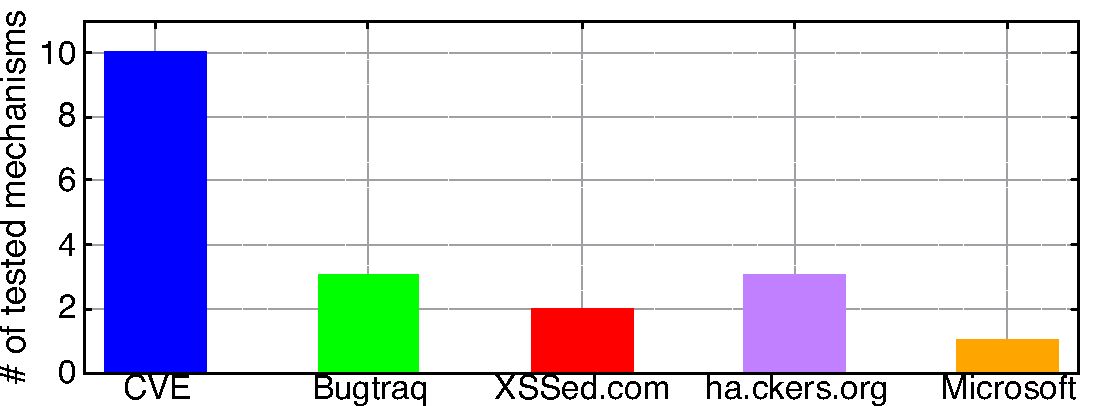
\includegraphics[scale=0.40]{barchart.pdf}
\end{center}
\vspace{-5.7mm}
\caption{\label{fig:defect_sources}Most common sources of real-world vulnerabilities
used for testing of web attack defenses.
Specifically, the publications that used a particular source are as follows:
{\sc cve}~\cite{XBS06,NLC07,PMP11,BK04,BV08,JB07,SMS13,WPLKK09,JKK06a,PS11},
Bugtraq~\cite{PB05,KJKV09,JEP08},
{\sc xss}ed.com~\cite{NSS06,APKLM10},
ha.ckers.org~\cite{TNH07,PSC09,LV09},
Microsoft~\cite{RDWDE07}.}
\vspace{-6.3mm}
\end{figure}

Table~\ref{tab:comp} indicates that the authors of 3 out of 35 (8.5\%)
publications provided a complete tuple of {\sc tp}, {\sc tn}, 
{\sc fp}, and {\sc fn}. On the other hand, we
see that 4 out of 35 (11.4\%) were not tested at all.
In these cases, all four elements of the tuple
are not available ({\sc na}). An interesting observation is
that in 10 out of the 35 (28.5\%)
publications, the evaluation focused on only on attack detection,
and there was no test focusing on false positives.
The corresponding tuples contain {\sc tp} and {\sc fn}
results, but {\sc tn} and {\sc fp} results are not available ({\sc
  na}). This stresses the fact that authors may be more interested in
making sure that their mechanisms can detect known attacks rather than
seeing how they respond under normal conditions. In some cases,
where the number of {\sc tp} results are not quantified, authors did
not mention how many or which attacks they performed. Moreover, in some
cases we observe that even if the authors report the existence of
possible false positive and negative results, they have not quantified
them ({\sc nq}).

Even when some numbers are given, they may not be adequate.
Sensitivity and specificity are statistical measures, and as such,
they should be interpreted with suitable confidence intervals. There are
various methods to calculate confidence intervals, even without
the need to have large sets of samples in order to be able to use the
central limit theorem~\cite{brown2001}.
However, sample sizes in the single
digits are not enough to produce good intervals.

Regarding the subjects of tests,
we see that 27 out of 35 (77.1\%)
mechanisms were tested with real-world
applications known to be vulnerable.
The vulnerabilities associated with these applications
are enlisted in the following providers: the Common
Vulnerabilities and Exposures ({\sc cve})
database,\footnote{\scriptsize\url{https://cve.mitre.org/}}
%~\cite{cve},
the Bugtraq\footnote{\scriptsize\url{http://seclists.org/bugtraq/}}
security mailing list,
%~\cite{bugtraq},
the {\sc xss}ed.com
security bulletin provider,\footnote{\scriptsize\url{www.xssed.com}}
%~\cite{xssed},
Microsoft's security
bulletin\footnote{\scriptsize\url{https://technet.microsoft.com/en-us/security/bulletin}}
%~\cite{microsoftBulletin}
and the
ha.ckers.org\footnote{\scriptsize\url{http://ha.ckers.org/}}
security bulletin provider.
%~\cite{hackers}.
Figure~\ref{fig:defect_sources},
presents how many,
and which, in the figure's caption, publications referred
to which source.
In numerous occasions authors performed tests based
on the same applications.
For example, 12 mechanisms were tested on a
vulnerable version of the {\sc phpbb} bulletin board
software.\footnote{\scriptsize\url{https://www.phpbb.com/}}
%~\cite{phpbb}.

There are also authors that took a different approach.
For instance, during their initial tests,
Stock et al.~\cite{SLMS14} managed to bypass
the browser-based {\sc xss} filters of
73\% out of 1,602 real-world {\sc dom}-based {\sc xss} vulnerabilities.
These vulnerabilities were actually found as part of
their previous research~\cite{LSJ13}.
Finally, in the {\sc amnesia}~\cite{HO05b} and
{\sc sd}river~\cite{MS09} publications,
the authors managed to break existing application suites
and then test the accuracy of their tools on them.

\subsection{Availability}

\begin{table}
\caption{Availability of the studied defenses.}
\vspace{-4mm}
    \label{tab:avail}
\centering
    \begin{threeparttable}
    \begin{small}
\scalebox{0.69}{
    \begin{tabular}{l|c|ccc}
    \thickhline
    \bf{Approach}
  & \bf{Mechanism}
  & \multicolumn{3}{c}{Availability\tnote{1}} \\
  && \bf{Source Code}
  & \bf{Executable}
  & \bf{Testbed} \\
    \thickhline
  \multirow{2}{*}{Parse-Tree Validation}
  &   {\sc sqlc}heck~\cite{SW06} & {\sc na} & {\sc na} & {\sc na} \\
  &   {\sc sqlg}uard~\cite{BWS05} & {\bf AO} & {\bf AO} & {\sc na} \\
  \hline
  \multirow{13}{*}{Policy Enforcement}
  &   {\sc dsi}~\cite{NSS06} & {\sc na} & {\sc na} & {\sc na} \\
  &   NoForge~\cite{JKK06a} & {\bf AO} & {\bf AO} & {\sc na} \\
  &   Noxes~\cite{KJKV09}  & {\sc na} & {\sc na} & {\sc na} \\
  % &   {\it {\sc met}}~\cite{ELX07} & {\sc na} & {\sc na} & {\sc na} \\
  &   {\sc beep}~\cite{TNH07} & \tick & \tick & \tick \\
  &   BrowserShield~\cite{RDWDE07} & {\sc na} & {\sc na} & {\sc na} \\
  &   CoreScript~\cite{YCIS07} & {\bf AO} & {\sc na} & {\sc na} \\
  &   {\sc soma}~\cite{OWVS08} & {\sc na} & {\sc na} & {\sc na} \\
  % &   {\it Barth et al.}~\cite{BJM08} & {\sc na} & {\sc na} & {\sc na} \\
  &   Phung et al.~\cite{PSC09} & \tick & \tick & \tick \\
  &   ConScript~\cite{ML10} & {\bf AO} & {\sc na} & {\sc na} \\
  &   CsFire~\cite{DDHPJ10} & \tick & {\sc na} & {\sc na} \\
  &   {\sc csp}~\cite{SSM10} & {\bf AO} & {\bf AO} & {\sc na} \\
  &   j{\sc csrf}~\cite{PS11} & {\sc na} & {\sc na} & {\sc na} \\
  &   WebJail~\cite{VDDPJ11} & {\sc na} & {\sc na} & {\sc na} \\
    % &   {\it {\sc js}and}~\cite{AVBPDP12} & {\sc na} & {\sc na} & {\sc na} \\
  % \hline
  % \hline 
  % \multirow{3}{*}{Securing Mashups}
  % &   {\it {\sc om}ash}~\cite{CHC08} & {\sc na} & {\sc na} & {\sc na} \\
  % &   {\it Mashup{\sc os}}~\cite{WFHJ07} & {\sc na} & {\sc na} & {\sc na} \\
  % &   {\it TreeHouse}~\cite{IW12} & {\sc na} & {\sc na} & {\sc na} \\
  \hline
  \multirow{4}{*}{{\sc isr}}
  &   {\sc sql}rand~\cite{BK04} & {\sc na} & {\sc na} & {\sc na} \\
  &   {\sc sm}ask~\cite{JB07} & {\sc na} & {\sc na} & {\sc na} \\
  &   Noncespaces~\cite{GC09} & {\sc na} & {\sc na} & {\sc na} \\
  &   x{\sc js}~\cite{APKLM10} & {\sc na} & {\sc na} & {\sc na} \\
  \thickhline
  \thickhline
  \multirow{7}{*}{Taint Tracking}
  &   Haldar et al.~\cite{HCF05}  & {\sc na} & {\sc na} & {\sc na} \\
  &   {\sc csse}~\cite{PB05} & {\sc na} & {\sc na} & {\sc na} \\
  &   Xu et al.~\cite{XBS06}  & {\sc na} & {\sc na} & {\sc na} \\
  &   {\sc wasc}~\cite{NLC07} & {\sc na} & {\sc na} & {\sc na} \\
  &   Vogt et al.~\cite{VFJKKV07}  & {\sc na} & {\sc na} & {\sc na} \\
  &   {\sc php} Aspis~\cite{PMP11} & {\bf AO} & {\sc na} & {\bf AO} \\
  &   Stock et al.~\cite{SLMS14} & {\sc na} & {\sc na} & {\sc na} \\
  \hline
  \multirow{6}{*}{Training}
  &   {\sc didafit}~\cite{LLW02} & {\sc na} & {\sc na} & {\sc na} \\
  &   {\sc amnesia}~\cite{HO05b} & {\sc na} & {\bf AO} & {\sc na} \\
  &   libAnomaly~\cite{VMV05} & {\bf ?} & {\bf ?} & {\bf ?} \\
  &   {\sc xssds}~\cite{JEP08} & {\sc na} & {\sc na} & {\sc na} \\
  &   {\sc swap}~\cite{WPLKK09} & {\sc na} & {\sc na} & {\sc na} \\
  &   {\sc sd}river~\cite{MS09,MKLS11} & \tick & \tick & {\sc na} \\
  \thickhline
  \thickhline
  \multirow{3}{*}{Hybrid}
  &   {\sc xss-guard}~\cite{BV08} & {\sc na} & {\sc na} & {\sc na} \\
  &   Blueprint~\cite{LV09} & {\bf ?} & {\bf ?} & {\bf ?} \\
  &   Diglossia~\cite{SMS13} & {\sc na} & {\sc na} & {\sc na} \\
  \thickhline

    \multicolumn{5}{p{12.4cm}}{%
       $^\textsuperscript{1}$A check mark (\tick) indicates that the publication
       includes a link to a page where the software is available.
       {\bf AO} (Available On-line) indicates
       that the software is available on-line but the
       address is not mentioned in the paper, which probably means that
       the it was made available after the publication. A question 
       mark ({\bf ?}) indicates that a link to the software
       was included in the publication but is now inaccessible.} \\
    \end{tabular}}
    \end{small}
    \end{threeparttable}
    \vspace{-6.5mm}
\end{table}

Table~\ref{tab:avail} presents our findings regarding the availability
of each mechanism in terms of source code and corresponding
executables. We also examined the availability of the testbeds
mentioned in each paper. We see that only 6 out of 35 (17.1\%) of the
publications provided a link to their mechanism and, 2 from these 6
web pages are currently not available. In 5 cases authors made either
the source code or their executables available after their paper got
published. In one case ({\sc csp}~\cite{SSM10}), the source was available before the
publication through the Mozilla community.
Regarding the availability of test materials, we see that
only 3 out of 35 (8.5\%) publications have currently their testbeds
available.

\subsection{Performance Overhead}

Table~\ref{tab:comp} shows the performance overhead of each mechanism.
In addition, it indicates if the overhead is incurred at the
server ({\sc s}) or at the client-side ({\sc c}). In almost half of
the approaches, 16 out of 35 (45.7\%), the overhead is provided as a
percentage, while in other cases, 7 our of 35 (20\%), the authors
provide the latency (in ms) that their mechanisms add to the
normal execution time of the protected application. Note that in some
cases, the times of normal executions are not provided,
so it is not possible to convert absolute
time measurements to percentage overheads. In 10 cases (28.5\%), the
overhead was either not available ({\sc na}) or not quantified ({\sc
  nq}). For {\sc php aspis}~\cite{PMP11}, its authors indicate that with
their mechanism, the execution time is doubled.

\subsection{Ease of Use}
\label{sec:deploy2}

Mechanisms in different categories face different deployment issues.
Consider the majority of mechanisms in the policy enforcement
subcategory. In most cases, developers should modify multiple
components to use each mechanism. Specifically, mechanisms like
BrowserShield~\cite{RDWDE07} and {\sc beep}~\cite{TNH07}
require modifications both on the server
and at the client. Thus, it would be difficult to be
adopted by both browser vendors and application developers. On the
other hand, there are cases where the policies introduced at the
server are enforced at the client-side, via a library embedded in the
server's response (i.e., Blueprint~\cite{LV09}).
Such an approach is convenient
as no modifications are needed at the client.

Extensive modifications in the application's source
code can also be a reason that can make a mechanism
difficult to use. {\sc sql}rand~\cite{BK04},
{\sc amnesia}~\cite{HO05b},
mechanisms of the parse-tree validation
subcategory, and mechanisms of the taint
tracking subcategory are such examples.
In the first three cases, programmers should modify every
code fragment that involves the execution of a query.
In the latter case they should also change
all the code fragments that involve user input handling. 

Finally, even though many of the mechanisms that involve
training are easy to deploy, they have a distinct disadvantage.
When the application is altered, mechanisms like
{\sc sd}river~\cite{MS09}
and {\sc xss-guard}~\cite{BV08} require a new training phase.
However, with the increased adoption of automated testing
and continuous integration frameworks, this phase could be
easily repeated.

\subsection{Security}

In our discussion of the various mechanisms in Section~\ref{sec:defs}, we
observed that some of them can be bypassed by attackers that know
the internals of their operation.
Still, the design of some mechanisms allows them to
be extended and become immune to the circumvention attacks they are
currently vulnerable to. For example, policy enforcement frameworks
based on JavaScript or {\sc html} rewriting can be extended
to detect attacks that leverage {\tt iframe} tags. This does not apply
to all mechanisms though. In particular, training mechanisms like {\sc
  didafit}~\cite{LLW02} and {\sc xss-guard}~\cite{BV08} must be
redesigned to detect the atacks we described in the related sections.

Taking the attackers' point of view, mimicry attacks can affect a
range of different mechanisms: they can be used to bypass mechanisms
in the hybrid category, as well as the policy enforcement and training
subcategories.

\subsection{Point of Detection}

Given the fact that the final steps of
{\sc dsl} injection and {\sc csrf} attacks take place
at the server-side, all mechanisms that detect
such attacks are placed at some point within the server-side infrastructure.
From the mechanisms that detect {\sc dsl} code injection
attacks, 3 out of 13 (23\%) do so at the level
of the {\sc rdbms} (Point {\sc db}).
The other 11 are based on interposing on {\sc api} calls related to output
vectors (Point {\sc dbal}).

For frameworks that deal with {\sc xss} attacks, we
see that attack prevention may take place either at the server or
the client-side. In the first case, a proxy is typically placed in front of the server
to examine the server's responses before they reach a user's 
browser. In the second case, a modified browser or a library that is
securely downloaded from the server checks the responses for potential
attacks. We find that the tendency so far is to create frameworks that
perform detection on the client-side: in particular, 14 out of 24
frameworks (58,3\%) detect {\sc xss} attacks at the
client-side. Note that the majority of the mechanisms that detect
such attacks on the server can also detect {\sc dsl} code
injection attacks (6 out of 10).

\section{Recommendations and Lessons Learned}
\label{sec:lessons-learned}

Our observations lead to some lessons and recommendations that
developers of new mechanisms may find helpful. In particular,
our observations
call for improvements in the accuracy of experimental testing
and code availability, while
aiming to reduce performance overheads and deployment hurdles.

\subsection{Improving Testing Accuracy}

One of our key findings indicates that many proposed defenses are
tested in a poor manner. In many cases, researchers tend to not provide
results on false positives or false negatives for their mechanisms
(where applicable).
Mere discussion on the existence of such results without quantifying
them also blurs the picture.

A reasonable argument would be that many mechanisms (especially the
ones coming from the etiological category), do not need to be
established purely through testing, since they provide systematic
arguments as to why their design is secure against attacks. In order
for this to hold, however, their implementation should be flawless
and precisely follow its specification, which may not
be the case in practice. Moreover, even mechanisms that detect attacks
based on their root cause, instead of their observed behavior, may still be
circumvented by evasive attacks.

When we introduced specificity and sensitivity in
Section~\ref{ssec:diagnostic-performance}, we deferred discussion of
\textsc{ppv} and \textsc{npv} to this point. These two relate to the
effectiveness of a detection mechanism in an actual production setting,
instead of a testbed. If an attack is detected in a production
environment, how much should we be worried? The answer is provided by
\textsc{ppv}. If no attack is detected in a production environment,
how relaxed should we be that no attack has indeed taken place? The
answer is provided by \textsc{npv}. We can calculate \textsc{ppv} and
\textsc{npv} with the following equations:

\vspace{0.5mm}
\noindent\begin{minipage}{0.5\linewidth}
\begin{equation}
\textsc{ppv} = \frac{\textsc{tp}}{\textsc{tp} + \textsc{fp}}
\end{equation}
\end{minipage}
\begin{minipage}{0.5\linewidth}
\begin{equation}
\textsc{npv} = \frac{\textsc{tn}}{\textsc{fn} + \textsc{tn}}
\end{equation}
\end{minipage}\par\vspace{\belowdisplayskip}

\noindent
Equations~\ref{eq:ppv-se-sp} and~\ref{eq:npv-se-sp} use true and false
positives and negatives, like equations~\ref{eq:sensitivity}
and~\ref{eq:specificity}. However, \textsc{tp}, \textsc{tn},
\textsc{fp}, and \textsc{fn} are not qualitatively the same in these two cases:
whereas sensitivity and specificity are measured on a testing
environment, \textsc{ppv} and \textsc{npv} are measured on a real,
production environment. In fact, if \textsc{pr} is the probability of
a particular class of attacks in the real world,
i.e., its prevalence, then we
have~\cite{linn2004}:

\begin{equation}
\textsc{ppv} = \frac{\textsc{se}\times \textsc{pr}}{
\textsc{se}\times \textsc{pr} + (1 - \textsc{sp})\times (1 -
\textsc{pr})}
\label{eq:ppv-se-sp}
\end{equation}

\begin{equation}
\textsc{npv} = \frac{\textsc{sp}\times (1 - \textsc{pr})}{
(1 - \textsc{se})\times \textsc{pr} + \textsc{sp}\times (1 -
\textsc{pr})}
\label{eq:npv-se-sp}
\end{equation}

\noindent
Prevalence is the prior probability that an event might be an attack,
based on our understanding of the volume and frequency of a particular
class of attacks; 
\textsc{ppv} and \textsc{npv} are the revised estimates of that
probability based on the results of the detection
mechanism. The lower the prevalence of an attack,
the more confident we can be that a negative test result indicates
that no attack has taken place and the less sure we can be that a
positive test result indicates a real attack. 

Of course it is not easy, and it may not even be possible, to know how
prevalent an attack class is. Also, attacks against a system may depend on
factors such as its visibility and popularity, and thus the same
software may be subject to varying attack intensity depending on
where it is actually deployed. With this in mind, it may be unfair to
ask researchers to provide \textsc{ppv} and \textsc{npv} values for
their mechanisms.
%---in fact, we observe that nobody does.

This does not mean though that deriving \textsc{ppv} and \textsc{npv} is
altogether impossible. One could deploy a system armoured with an
attack detection mechanism on a honeypot to study what happens over
a time period. This could give an indication about the performance of
the mechanism in a realistic setting. Alternatively, one could deploy a
target, unarmoured system, on a honeypot to study the prevalence of
the class of attacks to be detected. Studying the prevalence of
classes of attacks is an interesting area of study on its own,
and could feed directly on the evaluation of attack detection
mechanisms as practical tools.

Apart from demonstrating the value of a mechanism, good accuracy tests
may be beneficial per se, leading to more well-designed and robust
defenses. Mechanisms that can be circumvented were not extensively
tested in terms of accuracy. For instance, {\sc didafit}~\cite{LLW02}
was not tested at all and {\sc xss-guard}'s~\cite{BV08}
testing involved 6 known attacks.
This also applies to some frameworks coming from the taint tracking
subcategory. It is possible that more tests during development would
have led the authors to larger design improvements~\cite{Van14}.

The accuracy of a tool may be related to the scope of the attacks it
aims to detect. A more limited scope may allow the development of more
accurate tools. In this vein, the system by Stock et al~\cite{SLMS14}
is the only one that targets exclusively {\sc dom}-based {\sc xss}
attacks and detects them in an accurate manner, as seen in
Table~\ref{tab:comp}. It is also extensively tested with real-world
attacks.

\subsection{Code Availability}

Apart from testing practices, another area that merits improvement is
the availability of prototypes and testbeds. We are not aware of
specific reasons why authors of detection mechanisms seem to be
wary of publicly releasing their code and tests. Our finding may reflect
the status in the current point in time, when authors are urged to
publish their code and tests, and may start, or may have already
started doing so, but this does not show yet in the research we
examined, which goes several years back. We also saw instances where
material was published, but does not seem to be available any more.
That points to the importance of reproducibility of research materials, 
an issue arising in all scientific fields. It is not enough to
publish the underlying code and data, but to make sure that it remains
accessible, and to provide the means to test it even as technology
advances and operating systems, file formats, and software libraries
change. That may be too much to ask right now; what seems reasonable,
though, is to ask of researchers working on defenses not to
buck the trend and to take steps to increase the availability of their
research.

\subsection{Performance Overhead and Deployment Remarks}

Performance overhead comes up as a non-trivial issue. We observe
that there are some mechanisms that introduce an overhead
that is more than 10\%. Relative
research on protection mechanisms~\cite{SPWS13} indicates that
mechanisms that introduce an overhead larger than 10\% do not tend to
gain wide adoption in production environments. Hence, the
computational overhead of some mechanisms could be a reason why they
have not been adopted.

The deployment difficulties we have found with many mechanisms are not
a reason not to adopt them, but they may hinder their widespread use.
Since code injection attacks are complex, it may be logical to
expect that mechanisms to detect them would be complex too. The effort
to install and use a tool should be weighed against the expected
benefits. That is one more reason why it is important to report tool
accuracy, as this provides an immediate indicator to the expected
benefits. 

The issue is more acute when the point of detection is at the client.
We saw that many policy enforcement mechanisms that detect attacks at
the browser are not easy to deploy because modifications are needed
both on the server and the client-side.
Conversely, it may be possible to deliver
the tools to the user unobtrusively; for example, we saw that
Blueprint~\cite{LV09} enforces policies at the client-side by embedding a library
in the server's response to the client. In general, when developing a
new countermeasure, researchers should consider where it
will detect attacks, observe the corresponding deployment
challenges, and try to mitigate them.

\section{Conclusion}
\label{sec:conclusion}

Despite many approaches that have been developed,
attacks based on code injection against web applications
have been consistently present for the last 15 years,
and it appears that they will continue to be.
Attackers seem to find new ways to introduce
malicious code to applications using a
variety of languages and techniques~\cite{HNSHS12,DKH14}.
Meanwhile, during the last decade, there have been
numerous mechanisms designed to
detect one or more of types of such attacks.
Although some deployed and widely used frameworks, 
such as {\sc csp}~\cite{SSM10},
% and
% Google Caja,\footnote{\scriptsize\url{https://code.google.com/p/google-caja/}}%~\cite{M06},
share characteristics
(for instance, {\sc html} sanitization and {\tt eval} handling)
with previous proposals, 
most research works are still not used in practice.

In order for a security tool to be used in practice, it must provide
some value to the user. In particular, the value should outweigh the
cost of its use. The cost is not necessarily monetary, but may be
incurred from the time required to use the tool, any inconvenience
caused, false alarms that may raise, and so on. These costs are related to the
issues we have been investigating here: poor testing, high overhead,
lack of publicly available prototypes,
deployment difficulties, compromised security. 

Improving any of these aspects would not just increase the value of a 
research work as a practical tool, but it would also increase its
research value as well.
Accurate detection reporting would help in evaluating different
approaches. Extensive performance measurements can reveal impractical
designs and focus effort elsewhere. Availability of source code
enhances basic scientific tasks like verification and reproducibility. Ease of
deployment brings ease of experimentation. Secure methods can form the
basis for developing methods with more extensive coverage.

To the positive side, some defenses have been extensively tested in
terms of accuracy ({\sc sqlc}heck~\cite{SW06},
{\sc amnesia}~\cite{HO05b}, libAnomaly~\cite{VMV05}),
solve specific problems in an effective way
(Blueprint~\cite{LV09} and the system by Stock et al.~\cite{SLMS14}) or
have a low computational overhead
({\sc dsi}~\cite{NSS06} and the system by Phung et al.~\cite{PSC09}).
There are also cases where
researchers have made their code available ({\sc beep}~\cite{TNH07}
and {\sc sd}river~\cite{MS09}),
which can promote the development of better
mechanisms. This argument has been raised by others
researchers too~\cite{SPWS13}.
Furthermore, testing defenses in a production
setting could also propel their adoption.

We hope that the exploitation model, analysis, and observations that
emerged from our research can be a reference point for researchers who
aim to develop new, practical countermeasures against web application
attacks.

\bibliographystyle{IEEEtran}
\bibliography{questioning}

\section*{Author Biographies}
\noindent
{\bf Dimitris Mitropoulos} is a Postdoctoral Researcher
in the Computer Science Department
at Columbia University in the City of New York.
He holds a PhD ('14) in Cyber Security from the
Athens University of Economics and Business.
He is an {\sc ieee} member, a member of SysSec,
and an official writer for the
{\sc xrds}: Crossroads blog of {\sc acm}.
His research interests include application security,
systems security and software engineering.

\noindent
{\bf Panos Louridas} is an Associate Professor at
the Athens University of Economics and Business.
He has published in many areas of software engineering
and is actively involved in the application of security
research for the development of high-stakes production
systems, such as e-voting.

\noindent
{\bf Michalis Polychronakis} is an Assistant Professor
at Stony Brook University.
He received the B.Sc. ('03), M.Sc. ('05), and Ph.D. ('09)
degrees in Computer Science from the University of Crete, Greece.
% while working as a research assistant in the Distributed
% Computing Systems Lab at {\sc forth-ics}.
Before joining Stony Brook, he was an Associate Research
Scientist at Columbia University in the City of New York.
His research interests include
network and system security and network monitoring and measurement.

\noindent
{\bf Angelos D. Keromytis} is an Associate Professor
of Computer Science at Columbia University in the City
of New York, and the director of the Network Security Lab.
He is currently serving as  Program Manager with the
Information Innovation Office ({\sc i}2O) at the Defense Advanced
Research Projects Agency ({\sc darpa}),
part of the Department of Defense.
His research interests are in systems
and network security,
and cryptography.
He is an {\sc acm} Distinguished Scientist since 2012,
and a founder of Allure Security Technology Inc.

\end{document} 

